\chapter{Fn: Guía de usuario}
\label{chap:fn-guia}

En este capítulo voy a presentar mi aplicación desde el punto de vista del usuario. Hablaré sobre las características que tiene y cómo usarlas para desplegar una función. Además es la oportunidad perfecta para presentar algunas capturas que demuestren el aspecto visual de la interfaz que nos encontraremos al abrir la aplicación.

\section{Fnctl}

\emph{Fnctl} es la herramienta de línea de comandos. Es un binario único sin ninguna dependencia aparte de \emph{glibc} que llevan todos los sistemas Linux. Podemos dejarlo en cualquier carpeta que esté en el \emph{PATH} como \emph{/usr/bin/fnctl} o \emph{/usr/local/bin/fnctl}.

\subsection{Ayuda con los comandos disponibles}

Todo lo que hagamos con la herramienta se realiza ejecutando un comando o subcomando disponible. Podemos consultar cuáles existen usando \emph{fnctl --help} y explorando desde ahí, como se aprecia en las figuras \ref{fig:fnctl-help} y \ref{fig:fnctl-help-functions}.

\begin{figure}[H]
    \centering
    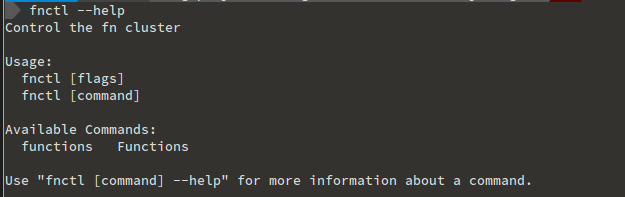
\includegraphics[width=\textwidth]{../images/fnctl/help.png}
    \caption{Salida de ayuda con \emph{fnctl --help}}
    \label{fig:fnctl-help}
\end{figure}

\begin{figure}[H]
    \centering
    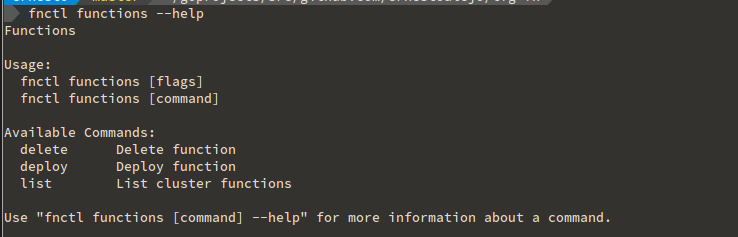
\includegraphics[width=\textwidth]{../images/fnctl/help-functions.png}
    \caption{Salida de ayuda con \emph{fnctl functions --help}}
    \label{fig:fnctl-help-functions}
\end{figure}

\subsection{Listar funciones}

Podemos listar las funciones que están desplegadas en estos momentos en el cluster. La salida es una tabla como la expuesta en la figura \ref{fig:fnctl-list}. En ella podemos apreciar ciertos datos generales como el script que vamos a llamar y qué trigger tiene activo para ejecutarla. Más adelante en la sección \ref{sec:trigger-http} veremos para qué sirve y como se ejecuta un trigger. Por último también nos dice cuanto tiempo ha estado la función activa en el cluster.

\smallskip

\begin{figure}[H]
    \centering
    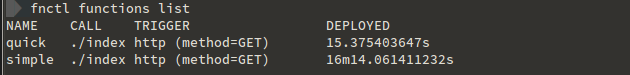
\includegraphics[width=\textwidth]{../images/fnctl/list.png}
    \caption{Listado de funciones desplegadas en el cluster}
    \label{fig:fnctl-list}
\end{figure}

\subsection{Despliegue de una nueva función}

La herramienta de línea de comandos es la única que puede desplegar una nueva función en el cluster a través del subcomando \emph{fnctl functions deploy}. Se le pasa como primer y único argumento el fichero de configuración en HCL; ver sección \ref{sec:hcl} más adelante para el formato.

\begin{figure}[H]
    \centering
    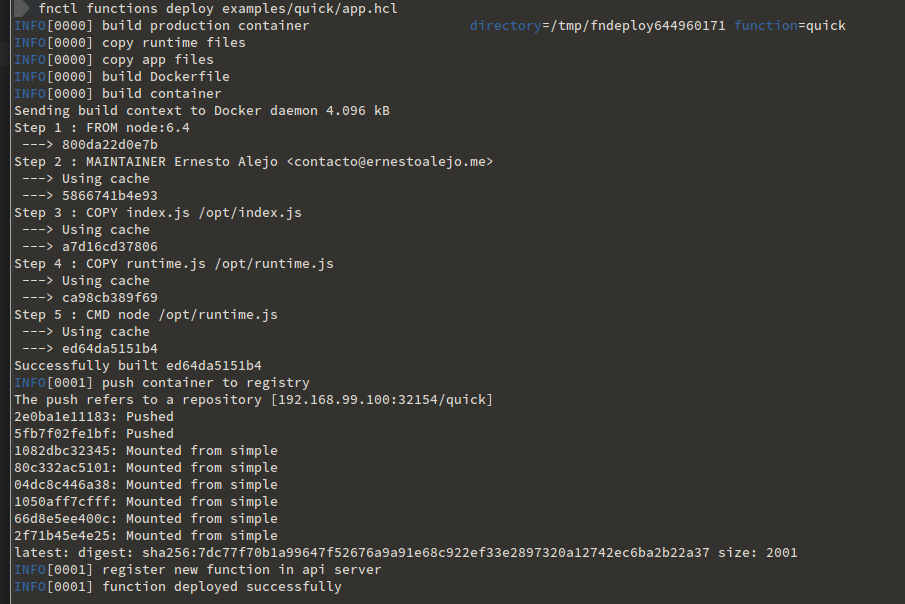
\includegraphics[width=\textwidth]{../images/fnctl/deploy.png}
    \caption{Despliegue de una nueva función}
    \label{fig:fnctl-deploy}
\end{figure}

Como vemos en la captura de la figura \ref{fig:fnctl-deploy} el despliegue está formado por varios pasos:
\begin{enumerate}
    \item Construir usando el demonio Docker local una imagen con la función que queremos ejecutar. Se busca una carpeta temporal donde se almacenarán los ficheros a construir y se ejecutan varios pasos sobre esa carpeta:
        \begin{enumerate}
            \item Copiar los ficheros de runtime del lenguaje elegido, Javascript por ejemplo.
            \item Copiar los ficheros de nuestra aplicación.
            \item Generar un Dockerfile para todos esos ficheros.
            \item Construir la imagen del contenedor.
        \end{enumerate}
    \item Con la imagen del contenedor ya preparada la enviamos al registro propio que tiene el cluster. En la figura se ve como alguna de las capas las ha reutilizado (\emph{Mounted from XXX}) de otra imagen que ya había en el cluster para optimizar la transferencia.
    \item Finalmente registra la nueva función con la API para que podamos empezar a servirla y utilizarla. A partir de este momento aparecerá en los listados.
\end{enumerate}

\subsection{Eliminar funciones}

La herramienta cierra el ciclo de despliegue de funciones con el comando para eliminarlas. Recibe como primer argumento el nombre de la función como reflejo en la figura \ref{fig:fnctl-delete}.

Si existe alguna instancia abierta de la función en el cluster iniciará el apagado de todas ellas inmediatamente de forma asíncrona.

\begin{figure}[H]
    \centering
    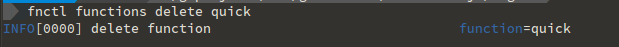
\includegraphics[width=\textwidth]{../images/fnctl/delete.png}
    \caption{Eliminar una función por línea de comandos}
    \label{fig:fnctl-delete}
\end{figure}

\section{Triggers}

Los \emph{triggers} son mecanismos que desencadenan una llamada a la función que hemos elegido. Son fáciles de implementar porque no usan ningún tipo de estado interno, así que se pueden añadir nuevos al código del sistema con facilidad como reflejaré en la sección \ref{sec:nuevos-triggers}.

\subsection{Trigger HTTP}
\label{sec:trigger-http}

Activa una llamada a la función desde una petición HTTP a una dirección determinada. Recoge los datos de la petición como cabeceras, URL y cuerpo y los mete en el contexto que recibe nuestra aplicación al ejecutarse. La respuesta de la función se envía como respuesta a la petición.

En las figuras \ref{fig:trigger-http} y \ref{fig:trigger-http2} vemos una petición a una función llamada \emph{simple} que devuelve el parámetro que le pasemos. El ejemplo de implementación lo veremos en la sección \ref{subsec:javascript}. En las capturas la IP corresponde a la que ha generado Minikube; en un cluster real se sustituiría por el balanceador de carga de las máquinas.

\begin{figure}[H]
    \centering
    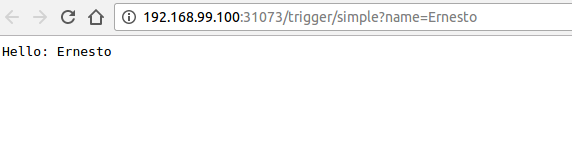
\includegraphics[width=\textwidth]{../images/output/ernesto.png}
    \caption{Trigger HTTP que devuelve el parámetro que le pasan}
    \label{fig:trigger-http}
\end{figure}

\begin{figure}[H]
    \centering
    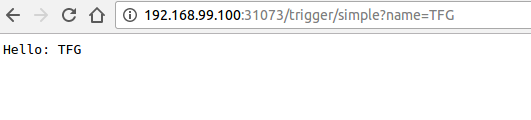
\includegraphics[width=\textwidth]{../images/output/tfg.png}
    \caption{Trigger HTTP probando con otro parámetro}
    \label{fig:trigger-http2}
\end{figure}

\section{Monitorización}

Una vez desplegadas las funciones podemos extraer a tiempo real estadísticas del funcionamiento desde esta pestaña del panel de control web. Los gráficos se actualizan continuamente sin tener que recargar la página y nos muestran la evolución del sistema en los últimos minutos.

En la figura \ref{fig:monitoring} podemos observar la gráfica que traza una función a medida que se crean o se destruyen instancias de acorde a la carga recibida. En la sección \ref{sec:load-test} analizaremos más en profundidad el comportamiento del sistema que viene reflejado aquí.

\begin{figure}[H]
    \centering
    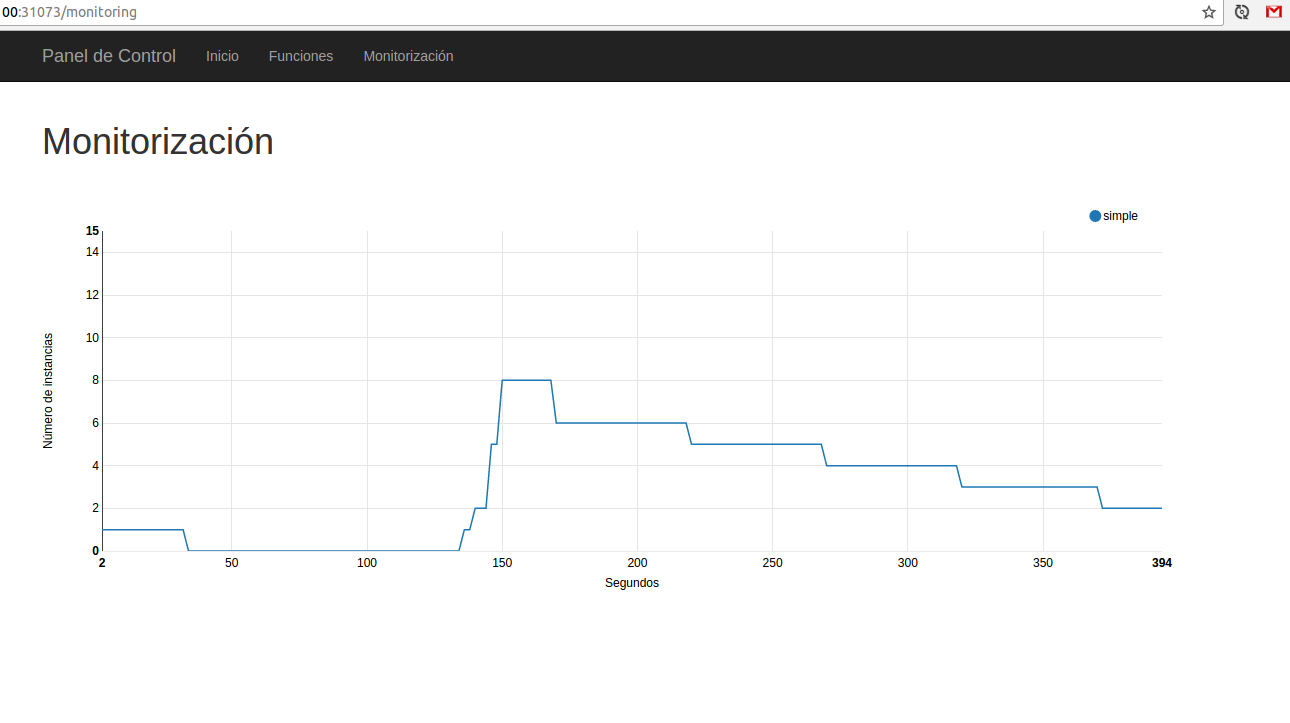
\includegraphics[width=\textwidth]{../images/fnapi/monitoring.png}
    \caption{Monitorización del número de instancias de una función}
    \label{fig:monitoring}
\end{figure}

\section{Configuración de la función: HCL}
\label{sec:hcl}

Para desplegar una función nos hace falta un pequeño fichero de configuración que determine ciertas variables a tiempo de ejecución del entorno; como el nombre, el fichero a ejecutar o el lenguaje de programación. Este fichero está escrito en un lenguaje muy sencillo llamado HCL\cite{hcl} que Hashicorp\cite{hashicorp} usa para productos como Terraform y Nomad\cite{nomad}.

El fichero debe describir el nombre de la función, el fichero a ejecutar, los ficheros que hay que desplegar y el tipo de trigger que queremos. Como mínimo hay que desplegar el fichero a ejecutar, aunque pueden seleccionarse otros que queramos incluir como plantillas, configuraciones propias, etc.

Aquí podemos observar un fichero de ejemplo que configura una función llamada \emph{simple} con un trigger HTTP:
\begin{minted}[baselinestretch=1.2]{text}
function {
  name = "simple"
  call = "./index"
  files = [
    "index.js",
  ]
  trigger = "http"
  method = "GET"
}
\end{minted}

\section{Implementación de la función}

La implementación se hace como una función nativa corriente del lenguaje. Recibirá como parámetros un contexto con información sobre la petición que dependerá del trigger y un objeto para devolver una respuesta al trigger si fuera necesario. Dentro de la función podemos llamar a otras, esperar a un petición externa, etc.; cualquier cosa y librería válida dentro del lenguaje.

\subsection{Javascript}
\label{subsec:javascript}

En el caso de Javascript debemos exportar una función en el módulo que seleccionemos en la configuración. Esa función recibirá la petición y el objeto para devolver la respuesta, al estilo de un simple handler de Express\cite{expressjs}.

El ejemplo más simple recibe un parámetro en la URL del trigger HTTP y lo emite concatenado a una cadena de texto:
\begin{minted}[baselinestretch=1.2]{javascript}
module.exports = function(request, response) {
  response.write(`Hello: ${request.form.name}`);
};
\end{minted}

Dentro del contenedor se ejecuta Node.js v4, con los que se pueden usar las nuevas construcciones de ES6 que ya estén disponibles en esa versión. En el ejemplo he usado literales con plantillas\cite{templateliterals} para sustituir el parámetro de la petición.

\section{Prueba de autoescalado}
\label{sec:load-test}

Una vez desplegada la función aparte de probar que funciona bien podemos ir un poco más allá y hacer pruebas con el autoescalado. El objetivo de este apartado no va a ser evaluar el rendimiento como tal, sino exclusivamente evaluar la funcionalidad de adaptación a los usuarios que lleguen. Para ello necesitamos generar cierta carga artificial. Lo normal sería usar herramientas como \emph{ab}\cite{ab}; pero la mayor parte de ellas no están bien diseñadas para el objetivo de medir carga real.

Las herramientas como \emph{ab} requieren un número total de peticiones y el número de conexiones concurrentes que pueden hacer. Eso significa que si pedimos 1000 peticiones y 10 procesos por ejemplo; cada uno de ellos irá pidiendo en paralelo de 10 en 10 hasta llegar al total. Éste no es un comportamiento propio de usuarios reales.

Para reproducir el tráfico más fielmente necesitamos una herramienta que mantenga un número de peticiones por segundo estable sin esperarse a que respondan; no porque una petición tarde 3 segundos otro usuario al otro lado del mundo iba a estar esperando para hacer la llamada. Podemos pedir por ejemplo 10 peticiones por segundos; si alguna de ellas no se procesa a lo mejor al segundo siguiente nos encontramos con 12 peticiones; y así hasta que el sistema gestione esa cola a una velocidad adecuada. He elegido Vegeta\cite{vegeta} para estas mediciones.

La elección de la herramienta es clave porque nos interesa ajustar el comportamiento cuando la carga cambia; si mantenemos una carga concurrente estable y serializada como la de \emph{ab} da lo mismo lo que hagamos porque siempre podemos regular los resultados a nuestro antojo según la velocidad de respuesta que tengamos. Al no medir la latencia total incluyendo el tiempo de cola de las peticiones el controlador de autoescalado abre menos instancias de las realmente necesarias.

He ejecutado \emph{vegeta} con 15 peticiones por segundo durante 30 segundos; y he reenderizado la salida con el informe HTML que lleva integrado. El resultado lo podemos observar en la figura \ref{fig:vegeta-plot}. Vemos como empieza con una latencia alta (eje Y) de unos 7 segundos por la cola tan profunda de peticiones que hay; a los 5/6 segundos empiezan a abrirse nuevas instancias y se aprecia como la latencia empieza a bajar rápidamente hasta alcanzar unos pocos milisegundos que es lo que tarda realmente en contestar (no hay tiempo de cola prácticamente).

\begin{figure}[H]
    \centering
    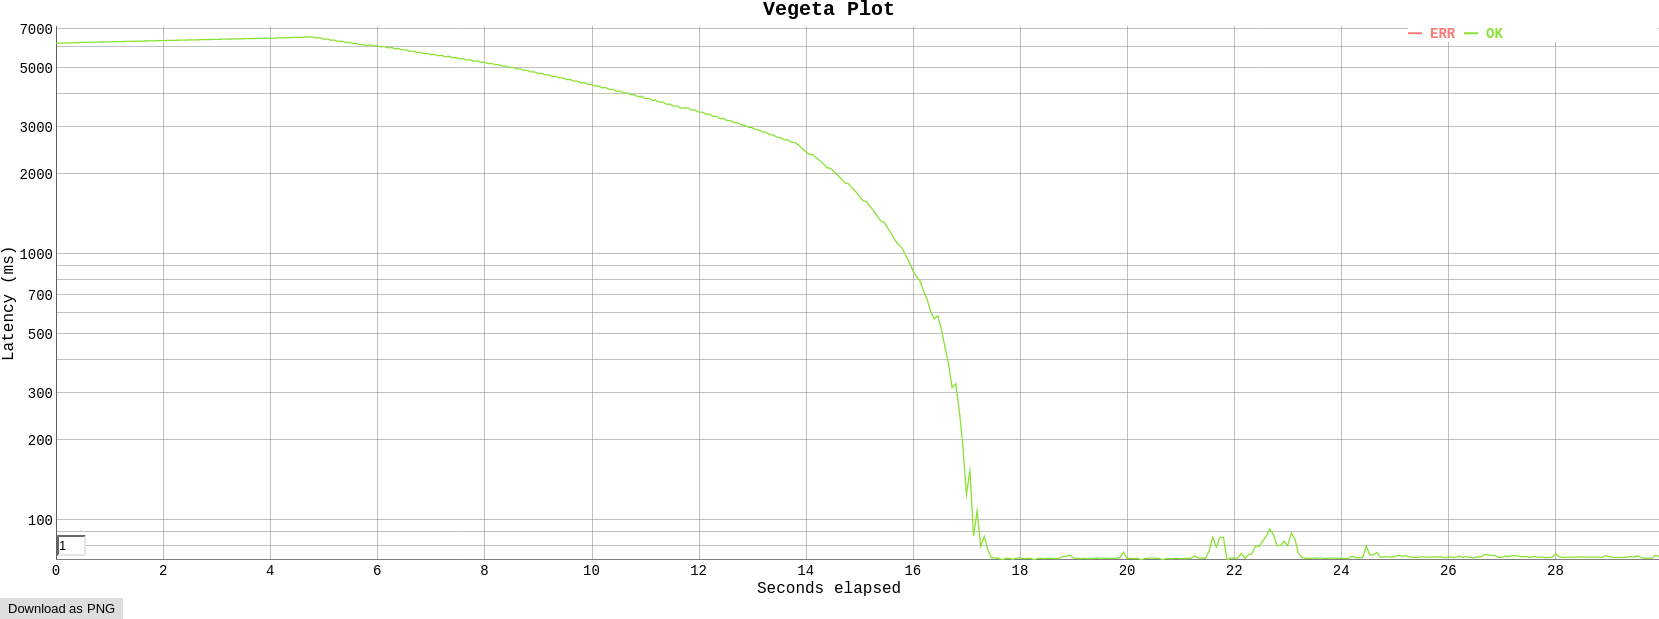
\includegraphics[width=\textwidth]{../images/fnapi/vegeta-plot.png}
    \caption{Resultado de la herramienta de pruebas de carga}
    \label{fig:vegeta-plot}
\end{figure}

La otra cara de la prueba de escalado la vemos en la monitorización del número de instancias que podemos obtener del panel de control web. Se aprecia un escalado muy rápido que da cabida a todo el tráfico entrante lo más pronto posible y que sube de cero instancias a 8 en cuestión de 15/20 segundos. Cuando la carga se acaba el sistema va retrocediendo más lentamente en capacidad hasta igualar la necesidad.

\begin{figure}[H]
    \centering
    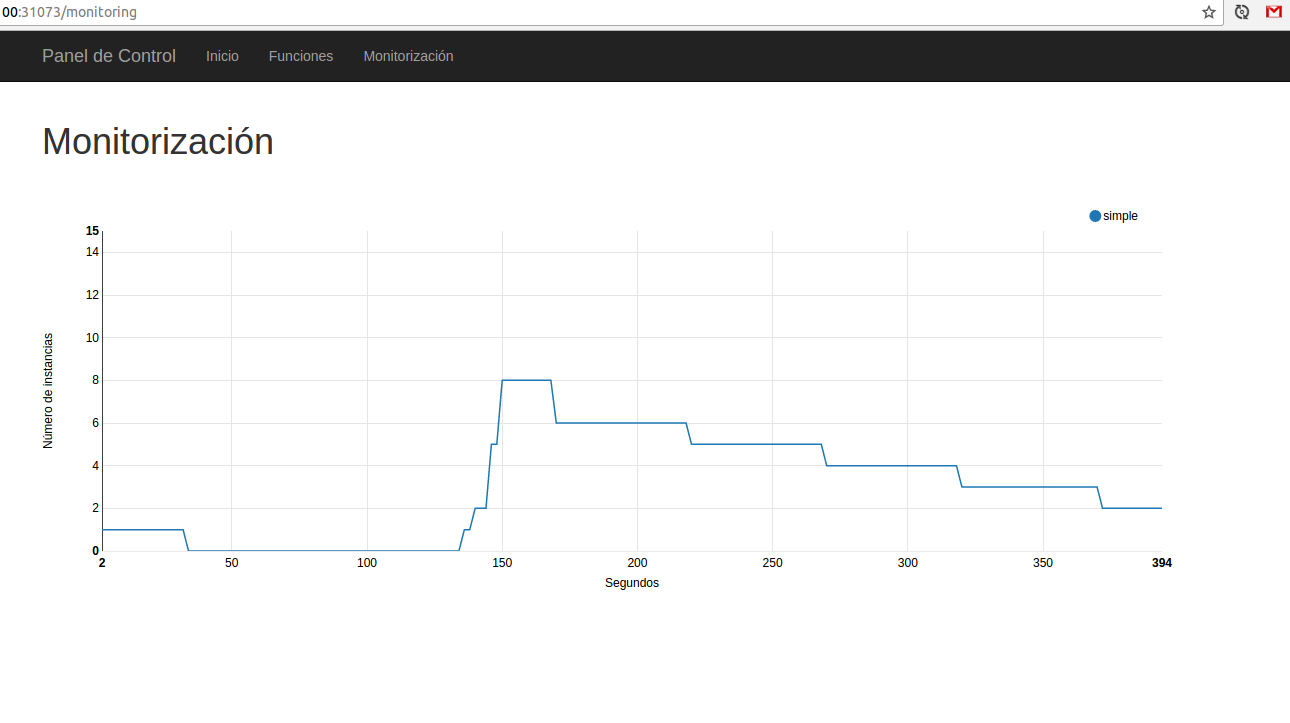
\includegraphics[width=\textwidth]{../images/fnapi/monitoring.png}
    \caption{Monitorización de la prueba de escalado}
    \label{fig:monitoring-scale}
\end{figure}

La bajada de capacidad está limitada artificialmente para intentar minimizar el efecto que tenga una carga desigual por picos en el número de instancias. Con mediciones de carga real seguramente sería recomendable examinar y ajustar esos valores para optimizar al máximo posible el gasto en servidores.
